\let\negmedspace\undefined
\let\negthickspace\undefined
\documentclass[journal,cmex10]{IEEEtran}
\usepackage[a5paper, margin=10mm, onecolumn]{geometry}
\usepackage{tfrupee}
\usepackage{cite}
\usepackage[cmex10]{amsmath}
\usepackage{amssymb}
\usepackage{amsfonts}
\usepackage{amsthm}
\usepackage{float}
\usepackage{algorithmic}
\usepackage{graphicx}
\usepackage{textcomp}
\usepackage{xcolor}
\usepackage{txfonts}
\usepackage{listings}


\usepackage{enumitem}
\setlistdepth{9}
\renewlist{enumerate}{enumerate}{9}
\setlist[enumerate,1]{label=\arabic*., leftmargin=*}
\setlist[enumerate,2]{label=\alph*), leftmargin=*}


\usepackage{mathtools}
\usepackage{gensymb}
\usepackage{comment}
\usepackage[breaklinks=true]{hyperref}
\usepackage{tkz-euclide}
\usepackage{circuitikz}
\usepackage{xparse}
\usepackage{siunitx}
\usepackage{mathrsfs}
\usepackage{stfloats}
\usepackage{steinmetz}
\usepackage{bm}
\usepackage{cases}
\usepackage{subfig}
\usepackage{longtable}
\usepackage{tabularx}
\usepackage{multirow}
\usepackage{lscape}
\usepackage{chngcntr}
\usepackage{color}
\usepackage{array}
\usepackage{calc}
\usepackage{hhline}
\usepackage{ifthen}
\usepackage{setspace}
\usepackage{float}
\usepackage{listings}
\usepackage{verbatim}

\usepackage{multicol}

\usetikzlibrary{calc,math}
\usetikzlibrary{fadings}

\setlength{\headheight}{1cm}
\setlength{\headsep}{0mm}
\setlength{\intextsep}{10pt}

\hyphenation{op-tical net-works semi-conduc-tor}
\def\inputGnumericTable{}

\lstset{
frame=single,
breaklines=true,
columns=fullflexible
}

\providecommand{\pr}[1]{\ensuremath{\Pr\left(#1\right)}}
\providecommand{\qfunc}[1]{\ensuremath{Q\left(#1\right)}}
\providecommand{\sbrak}[1]{\ensuremath{{}\left[#1\right]}}
\providecommand{\lsbrak}[1]{\ensuremath{{}\left[#1\right.}}
\providecommand{\rsbrak}[1]{\ensuremath{{}\left.#1\right]}}
\providecommand{\brak}[1]{\ensuremath{\left(#1\right)}}
\providecommand{\lbrak}[1]{\ensuremath{\left(#1\right.}}
\providecommand{\rbrak}[1]{\ensuremath{\left.#1\right)}}
\providecommand{\cbrak}[1]{\ensuremath{\left\{#1\right\}}}
\providecommand{\lcbrak}[1]{\ensuremath{\left\{#1\right.}}
\providecommand{\rcbrak}[1]{\ensuremath{\left.#1\right\}}}
\theoremstyle{remark}
\newtheorem{rem}{Remark}
\providecommand{\abs}[1]{\ensuremath{\left\vert#1\right\vert}}
\providecommand{\res}[1]{\Res\displaylimits_{#1}}
\providecommand{\norm}[1]{\ensuremath{\left\lVert#1\right\rVert}}
\providecommand{\mtx}[1]{\mathbf{#1}}

\providecommand{\mean}[1]{\ensuremath{E\left[ #1 \right]}}

\providecommand{\dec}[2]{\ensuremath{\overset{#1}{\underset{#2}{\gtrless}}}}
\providecommand{\prt}[2]{\ensuremath{p_{#1}^{\left(#2\right)} }}
\newcommand{\sgn}{\mathop{\mathrm{sgn}}}
\providecommand{\cond}[2]{#1\middle|#2}
\let\vec\mathbf
\DeclareMathOperator*{\Res}{Res}
\newcommand{\solution}{\noindent \textbf{Solution: }}
\newcommand{\cosec}{\,\text{cosec}\,}
\newcommand{\myvecf}[2][0pt]{\ensuremath{\begin{pmatrix}\renewcommand{\arraystretch}{1.5}\def\myvec@rowspacing{#1}#2\end{pmatrix}}}
\newcommand{\myvec}[1]{\ensuremath{\begin{pmatrix}#1\end{pmatrix}}}
\newcommand{\augvec}[3]{\ensuremath{\begin{amatrix}{#1|#2}#3\end{amatrix}}}
\newcommand{\mydet}[1]{\ensuremath{\begin{vmatrix}#1\end{vmatrix}}}
\providecommand{\rank}{\text{rank}}
\providecommand{\gauss}[2]{\mathcal{N}\ensuremath{\left(#1,#2\right)}}
\providecommand{\diff}[2]{\ensuremath{\frac{d{#1}}{d{#2}}}}

\providecommand{\myceil}[1]{\ensuremath{\left\lceil #1 \right\rceil}}


\newcommand\figref{Fig.~\ref}
\newcommand\appref{Appendix~\ref}
\newcommand\probref{Problem~\ref}
\newcommand\tabref{Table~\ref}
\newcommand{\sinc}{\,\text{sinc}\,}
\newcommand{\rect}{\,\text{rect}\,}
\newcommand*{\permcomb}[4][0mu]{{{}^{#3}\mkern#1#2_{#4}}}
\newcommand*{\perm}[1][-3mu]{\permcomb[#1]{P}}
\newcommand*{\comb}[1][-1mu]{\permcomb[#1]{C}}
\let\define\triangleq

\newtheorem{theorem}{Theorem}[section]
\newtheorem{problem}{Problem}
\newtheorem{proposition}{Proposition}[section]
\newtheorem{lemma}{Lemma}[section]
\newtheorem{corollary}[theorem]{Corollary}
\newtheorem{example}{Example}[section]
\newtheorem{definition}[problem]{Definition}

\renewcommand\thesection{\arabic{section}}
\renewcommand\thesubsection{\thesection.\arabic{subsection}}
\renewcommand\thesubsubsection{\thesubsection.\arabic{subsubsection}}
\renewcommand\thesectiondis{\arabic{section}}
\renewcommand\thesubsectiondis{\thesectiondis.\arabic{subsection}}
\renewcommand\thesubsubsectiondis{\thesubsectiondis.\arabic{subsubsection}}
\setlist[enumerate,1]{label=\arabic*.}
\NewDocumentEnvironment{amatrix}{>{\SplitArgument{1}{|}}m}
  {\ensuremath{\left(
    \begin{array}{c}
      \makeamatrix#1
    \end{array}
    \right)}}
  
\NewDocumentCommand{\makeamatrix}{mmm}{%
  \IfNoValueTF{#2}
    {\ensuremath{\begin{array}{@{}*{#1}{c}@{}} #3 \end{array}}}
    {\ensuremath{\begin{array}{@{}*{#1}{c}|*{#2}{c}@{}} #3 \end{array}}}% 
    }

\NewDocumentCommand{\system}{gg}{%
  \IfNoValueTF{#1}
    {%
 \longleftrightarrow
    }
    {%
      \IfNoValueTF{#2}
      {%
\overset{\mathcal{#1}}{ \longleftrightarrow}
      }
      {%
\overset{\mathcal{#1}^{#2}}{ \longleftrightarrow}
      }
    }%
}

\newcounter{matchleft}\newcounter{matchright}
\newenvironment{matchtabular}{%
  \setcounter{matchleft}{0}%
  \setcounter{matchright}{0}%
  \tabularx{\textwidth}{%
    >{\leavevmode\hbox to 1.5em{\stepcounter{matchleft}\arabic{matchleft}.}}X%
    >{\leavevmode\hbox to 1.5em{\stepcounter{matchright}\alph{matchright})}}X%
    }%
}{\endtabularx}

\renewcommand{\thefigure}{\theenumi}
\renewcommand{\thetable}{\theenumi}
\numberwithin{equation}{enumi}
\numberwithin{figure}{enumi}

\begin{document}
\bibliographystyle{IEEEtran}
\vspace{3cm}

\title{GATE XE 2007}
\author{AI25BTECH11003 - Bhavesh Gaikwad}
{\let\newpage\relax\maketitle}

\section*{Section A: Engineering Mathematics (Compulsory)}
\vspace{2\baselineskip}
\begin{enumerate}

    \item Let $M =\myvec{ 1 & 1 & 1 \\ 0 & 1 &1 \\ 0 & 0 &1}$. Then the maximum number of linearly independent eigenvectors of M is:
    \hfill{(GATE 2007 XE)}
    
    \begin{multicols}{4}
    \begin{enumerate}
        \item 0
        \item 1
        \item 2
        \item 3
     \end{enumerate}
     \end{multicols}

    
    \item Let $ lim_{x \to \frac{\pi}{2}} \frac{\sin^{2}(2x)}{\left(x - \frac{\pi}{2}\right)^{2}} $. Then L is equal to :
    \hfill{(GATE 2007 XE)}
    \begin{multicols}{4}
    \begin{enumerate}
        \item -4
        \item 0
        \item 2
        \item 4
    \end{enumerate}
\end{multicols}


    \item Let $ f(z) = \frac{1}{1 - z^{2}} $. The coefficient of  $ f(z) = \frac{1}{z-1} $ in the Laurent expansion of f(z) about z=1 is:
    \hfill{(GATE 2007 XE)}
    \begin{multicols}{4}
    \begin{enumerate}
        \item -1
        \item $-\frac{1}{2}$
        \item $\frac{1}{2}$
        \item 1
    \end{enumerate}
\end{multicols}
    

    \item Let u(x,t) be the solution of the initial value problem $ \dfrac{\partial^{2}u}{\partial t^{2}} = 9,\dfrac{\partial^{2}u}{\partial x^{2}},; t>0,; -\infty<x<\infty $
$ u(x,0)=x+5,; \left.\dfrac{\partial u}{\partial t}\right|(x,0)=0 $. Then u(2,2) is:
    \hfill{(GATE 2007 XE)}
    \begin{multicols}{4}
        \begin{enumerate}
        \item 7
        \item 13
        \item 14
        \item 26
    \end{enumerate}
\end{multicols}

    \item Two students take a test consisting of five TRUE/FALSE questions. To pass the test the students have to answer at least three questions correctly. Both of them know the correct answers to two questions and guess the answers to the remaining three. The probability that only one student passes the test is equal to:
    \hfill{(GATE 2007 XE)}
    \begin{multicols}{4}
    \begin{enumerate}
    
        \item $\frac{6}{32}$
        \item $\frac{7}{32}$
        \item $\frac{1}{4}$
        \item $\frac{3}{4}$
    \end{enumerate}
    \end{multicols}

    \item The equation g(x) = x is solved by Newton-Raphson iteration method, starting with an initial approximation $x_n$ near the simple root a. If $x_{n+1}$ is the approximation to a at the (n+1)th iteration, then:

    \hfill{(GATE 2007 XE)}
    \begin{multicols}{4}
    \begin{enumerate}
        \item $ x_{n+1}=\frac{x_n\,g'(x_n)-g(x_n)}{1-g'(x_n)} $
        \item $ x_{n+1}=\frac{x_n,g'(x_n)-g(x_n)}{g'(x_n)-1} $
        \item $ x_{n+1}=g(x_n) $
        \item $ x_{n+1}=\frac{x_n,g'(x_n)-g(x_n)+2x_n}{g'(x_n)+1} $
    \end{enumerate}
\end{multicols}

    \item Let Ax = b be a system of m linear equations in n unknowns with m < n and $b \neq 0$. Then the system has:
  
    \hfill{(GATE 2007 XE)}
    \begin{multicols}{4}
    \begin{enumerate}
        \item n - m  solutions
        \item either zero or infinitely many solutions
        \item exactly one solution
        \item n  solutions
    \end{enumerate}
\end{multicols}

    \item Let R be an $n \times n $ nonsingular matrix. Let P and Q be two  $n \times n $ matrices such that $ Q = R^{-1}PR $. If x  is an eigenvector of  P corresponding to a nonzero eigenvalue $\lambda$ of P, then:
    \hfill{(GATE 2007 XE)}
    \begin{multicols}{4}
    \begin{enumerate}
        \item Rx  is an eigenvector of Q  corresponding to eigenvalue $\lambda$ of  Q 
        \item  Rx  is an eigenvector of Q  corresponding to eigenvalue $ \frac{1}{\lambda} $ of Q 
        \item $R^{-1}x$  is an eigenvector of Q  corresponding to eigenvalue $\lambda$ of Q 
        \item $ R^{-1}x$ is an eigenvector of Q  corresponding to eigenvalue $ \frac{1}{\lambda} $ of Q 
    \end{enumerate}
\end{multicols}

    \item Let M  be a $2 \times 2$ matrix with eigenvalues 1 and 2. Then  $ M^{-1}$ is:
    \hfill{(GATE 2007 XE)}
    \begin{multicols}{4}
    \begin{enumerate}[label=\alph*)]
        \item $M - 3I$
        \item $3I - M$
        \item $2I - M$
        \item $M^{-1} - 3I$
    \end{enumerate}
\end{multicols}

    \item The number of $n \times n$ matrices that are simultaneously Hermitian, unitary and diagonal is:
    \hfill{(GATE 2007 XE)}
    \begin{multicols}{4}
    \begin{enumerate}[label=\alph*)]
        \item $2^n$
        \item $n^2$
        \item $2n$
        \item 2
    \end{enumerate}
    \end{multicols}

    \item Let $M = \myvec{ 1 & b & a \\ 0 & 2 & c \\ 0 & 0 & 1}$, where  a, b, c are real numbers. Then M is diagonalizable:    
    \hfill{(GATE 2007 XE)}
    \begin{multicols}{4}
    \begin{enumerate}
        \item for all values of a, b, c
        \item only when $bc \neq a$
        \item only when b + c = a 
        \item only when bc = a
    \end{enumerate}
\end{multicols}

    \item The maximum value of the function 2x + 3y + 4z  on the ellipsoid $2x^2 + 3y^2 + 4z^2 = 1$ is:
    
    \hfill{(GATE 2007 XE)}
    \begin{multicols}{4}
    \begin{enumerate}
        \item 2
        \item 3
        \item 6
        \item 9
    \end{enumerate}
\end{multicols}

    \item Let $f: \mathbb{R} \to \mathbb{R}$ be a twice differentiable real valued function such that $f\left(\frac{1}{n}\right) = 1$ for  $n = 1, 2, 3, \dots$. Then:
\hfill{(GATE 2007 XE)}
\begin{multicols}{4}
    \begin{enumerate}
        \item $f'(0) = 0$
        \item  $f'(0) = 1$
        \item $0 < f'(0) < 1$
        \item $f'(0) > 1$
    \end{enumerate}
\end{multicols}

    \item Let $f(x) = \int_{0}^{\sqrt{x}} \sin t \, dt$ for  $x \geq 0$. Then $f'\left(\frac{x}{2}\right)$ is equal to:
    \hfill{(GATE 2007 XE)}
    \begin{multicols}{4}
    \begin{enumerate}
        \item 0
        \item $\pi$
        \item 1
        \item $\frac{\pi}{2}$
    \end{enumerate}
\end{multicols}

    \item The value of the contour integral $\oint_{|z|=1} \frac{4z^2 + 1}{\cosh z} \, dz$ is equal to:
    \hfill{(GATE 2007 XE)}
\begin{multicols}{4}
    \begin{enumerate}
        \item $2\pi i \cosh(i/2)$
        \item $\pi \cosh(i/2)$
        \item 0
        \item $2\pi i$
    \end{enumerate}
    \end{multicols}

    \item Let  $f(x+iy) = u(x,y) + iv(x,y)$ be an analytic function defined on the complex plane satisfying $2u^2 + 3v^2 = 1$. Then:
    \hfill{(GATE 2007 XE)}
    \begin{multicols}{4}
    \begin{enumerate}
        \item  f  is a constant
        \item f(z) = kz for some nonzero real k 
        \item $u(x,y) = \frac{\cos(x+y)}{\sqrt{2}}$
        \item $v(x,y) = \frac{\sin(x-y)}{\sqrt{3}}$
    \end{enumerate}
\end{multicols}

    \item The value of $\oint_C \left( xy^2 + 2x \right) dx + \left( x^2 y + 4x \right) dy$ along the circle $C: x^2 + y^2 = 4$ in the anticlockwise direction is:
    \hfill{(GATE 2007 XE)}
    \begin{multicols}{4}
    \begin{enumerate}
        \item $-16\pi$
        \item $-4\pi$
        \item $4\pi$
        \item $16\pi$
    \end{enumerate}
\end{multicols}

    \item The volume of the prism whose base is the triangle in the xy-plane bounded by the x-axis and the lines y = x and x = 2 , and whose top lies in the plane z = 5 - x - y is:
    \hfill{(GATE 2007 XE)}
    \begin{enumerate}[label=\alph*)]
        \item 2
        \item 4
        \item 6
        \item 10
    \end{enumerate}

    \item The general solution of $x \frac{\partial z}{\partial x} (z^2 - y^2) + (x - 2) \frac{\partial z}{\partial y} = (-x) \frac{\partial z}{\partial z}$ is:
    \hfill{(GATE 2007 XE)}
    \begin{multicols}{4}
    \begin{enumerate}
        \item $F(x^2 + y^2 + z^2, xyz) = 0$
        \item $F(x^2 + y^2 - z^2, xyz) = 0$
        \item $F(x^2 - y^2 + z^2, xyz) = 0$
        \item $F(-x^2 + y^2 + z^2, xyz) = 0$
    \end{enumerate}
    \end{multicols}

    \item Choose a point uniformly at random on the disc $x^2 + y^2 \leq 1$. Let the random variable X denote the distance of this point from the center of the disc. Then the variance of X is:
    \hfill{(GATE 2007 XE)}
    \begin{multicols}{4}
    \begin{enumerate}
        \item $\frac{1}{16}$
        \item $\frac{1}{17}$
        \item $\frac{1}{18}$
        \item $\frac{1}{19}$
    \end{enumerate}
\end{multicols}

\newpage

    \item If Runge–Kutta method of order 4 is used to solve the differential equation $\frac{dy}{dx} = f(x)$, y(0) = 0, in the interval [0,h] with step size h, then
    \hfill{(GATE 2007 XE)}
    \begin{multicols}{2}
    \begin{enumerate}
        \item $y(h) = \frac{h}{6} [f(0) + 4f(h/2) + f(h)]$
        \vspace{0.1cm}
        \item $y(h) = \frac{h}{6} [f(0) + f(h)]$
        \item $y(h) = h [f(0) + f(h)]$
        \item $y(h) = \frac{h}{6} [f(0) + 2f(h/2) + f(h)]$
    \end{enumerate}
\end{multicols}

    \item If a polynomial of degree three interpolates a function f(x) at the points (0,3), (1,13), (3,99), (4,187), then f(2) is:
    \hfill{(GATE 2007 XE)}
    \begin{multicols}{4}
    \begin{enumerate}
        \item 20
        \item 36
        \item 43
        \item 58
    \end{enumerate}
\end{multicols}

    \item Let $f(x) = x^2$ for $-\pi \leq x \leq \pi$ and f(x+2$\pi$) = f(x). The Fourier series of f in $[-\pi,\pi]$ is:
    \hfill{(GATE 2007 XE)}
    \begin{multicols}{2}
    \begin{enumerate}
        \item $\frac{\pi^2}{3} + 4 \sum_{n=1}^{\infty} \frac{\cos nx}{n^2}$
        \item $\frac{\pi^2}{3} + 4 (-1)^n \sum_{n=1}^{\infty} \frac{\cos nx}{n^2}$       
        \item $\frac{\pi^2}{3} + 4 (-1)^n \sum_{n=1}^{\infty} \frac{\cos nx}{n^2}$
        \item $\frac{\pi^2}{3} + \sum_{n=1}^{\infty} \frac{\cos nx}{n^2}$
    \end{enumerate}
\end{multicols}

    \item The sum of the absolute values of the Fourier coefficients of f is:
    \hfill{(GATE 2007 XE)}
    \begin{multicols}{4}
    \begin{enumerate}
        \item $\frac{\pi^2}{6}$
        \item $\frac{\pi^2}{3}$
        \item $\frac{2\pi^2}{3}$
        \item $\pi^2$
    \end{enumerate}
    \end{multicols}

    \item Let $y(x) = \sum_{n=0}^{\infty} a_n x^n$ be a solution of $ \frac{d^2 y}{dx^2} + x y = 0$. The value of $a_n$ is:\\
    \hfill{(GATE 2007 XE)}
    \begin{multicols}{4}
    \begin{enumerate}
        \item 0
        \item 1
        \item 2
        \item 3
    \end{enumerate}
\end{multicols}

    \item The solution of the above differential equation satisfying y(0) = 1 and y'(0) = 0 is:
    \hfill{(GATE 2007 XE)}
    \begin{multicols}{2}
    \begin{enumerate}
        \item $y(x) = 1 + \frac{x^2}{2! \cdot 3} - \frac{x^4}{2 \cdot 3 \cdot 5 \cdot 6} + \dots$
        \item  $y(x) = 1 - \frac{2 \cdot 3 x^2}{1} + \dots$
        \item $y(x) = 1 + \dots$
        \item $y(x) = 1 - \dots$
    \end{enumerate}
\end{multicols}

    \item The potential u(x,y) satisfies $\frac{\partial^2 u}{\partial x^2} + \frac{\partial^2 u}{\partial y^2} = 0$ in $0 \le x \le \pi$ , $0 \le y \le \pi$, with u = 0 on x = 0 ,  $x = \pi$ , y = 0 and nonzero at $y = \pi$. The potential is:
    \hfill{(GATE 2007 XE)}
    \begin{multicols}{2}
    \begin{enumerate}
        \item $u = \sum A_n \cosh(nx) \sin(ny)$
        \item $u = \sum A_n \sin(nx) \cosh(ny)$
        \item $u = \sum A_n \sinh(nx) \sin(ny)$
        \item $u = \sum A_n \sin(nx) \sinh(ny)$
    \end{enumerate}
\end{multicols}

    \item If  $y = \pi$ edge is at potential sin(x), then:
    \hfill{(GATE 2007 XE)}
    \begin{multicols}{2}
    \begin{enumerate}
    
        \item $u = \frac{\sin(nx) \sinh(ny)} {\sinh(n\pi)}$
        \item $u = \frac{\sin x \sinh y} {\sinh \pi}$
        \item $u = \frac{\sin x \cosh y} {\cosh \pi}$
        \item  $u = \frac{\cosh(nx) \sin(ny)} {\cosh(n\pi)}$
    \end{enumerate}
\end{multicols}


\end{enumerate}
    \vspace{3\baselineskip}
    \begin{center}
    \textbf{\Large ---END OF SECTION---}
    \end{center}

\newpage

\section*{Section B: Computational Science}
\vspace{2\baselineskip}
\begin{enumerate}[label=\arabic*)]

    \item If the 7-base representation of a number is 123, then its octal representation is\\
   \hfill{(GATE 2007 XE)}
   \begin{multicols}{4}
    \begin{enumerate}
        \item 102
        \item 103
        \item 111
        \item 112
    \end{enumerate}
    \end{multicols}

    \item Consider the following four FORTRAN statements: \\
    S1: X = 5**3 \\
    S2: X = (-5)**3.0 \\
    S3: X = 5**-3 \\
    S4: X = 5**3.0 \\
    Which of the following sets contains the valid statements from above?\\
    \hfill{(GATE 2007 XE)}
    \begin{multicols}{4}
    \begin{enumerate}
        \item \{S1, S3\}
        \item \{S1, S4\}
        \item \{S2, S3\}
        \item \{S2, S4\}
    \end{enumerate}
    \end{multicols}

    \item Which of the following sets contains the set of the basic data types in C?\\
    \hfill{(GATE 2007 XE)}
    \begin{multicols}{2}
    \begin{enumerate}
        \item \{char, int, float, logical\}
        \item \{char, boolean, int, float\}
        \item \{char, int, long, short, float, double\}
        \item \{char, int, float, void\}
    \end{enumerate}
\end{multicols}

    \item If a root of $f(x) = x^2 - 2x + 1 = 0$ is obtained by using iteration $x_{n+1} = x_n - \frac{f(x_n)}{f'(x_n)}$ with $x_0 = 0.5$, the convergence rate is\\
   \hfill{(GATE 2007 XE)}
   \begin{multicols}{4}
    \begin{enumerate}
        \item 1
        \item 1.62
        \item 1.84
        \item 2
    \end{enumerate}
\end{multicols}

    \item Let $S_1$ be the sum of the eigenvalues of a $2 \times 2$ matrix P and $S_2$ the sum of eigenvalues of another $2 \times 2$ matrix Q. If $S_1 = S_2$, then P and Q  are:
    \hfill{(GATE 2007 XE)}
    \begin{multicols}{2}
    \begin{enumerate}
        \item $\myvec{4 & 1 \\ 3 & 5}$ and $\myvec{ 3 & 2 \\ 3 & 5}$
        \item $\myvec{3 & 4 \\ 5 & 1 }$ and $\myvec{3 & 4 \\ 5 & 1 }$
        \item $\myvec{4 & 1 \\ 3 & 5 }$ and $\myvec{3 & 1 \\ 5 & 1 }$
        \item $\myvec{4 & 3 \\ 5 & 5 }$ and $\myvec{4 & 3 \\ 5 & 5 }$
    \end{enumerate}
\end{multicols}

    \item If $y_i$ denotes the value of y(x) at x = $x_i$ in  $x_0 < x_1 < \dots < x_n$, $x_i - x_{i-1} = h$ for $1 \le i \le n$, then  $\frac{d^2 y}{dx^2}$ at $x = x_i$ is approximated using finite differences by:\\
    \hfill{(GATE 2007 XE)}
    \begin{multicols}{4}
    \begin{enumerate}
        \item $\frac{y_{i+1} - 2y_i + y_{i-1}}{h^2}$
        \vspace{0.1cm}
        \item $\frac{y_{i+1} - y_i + y_{i-1}}{h^2}$
        \vspace{0.1cm}
        \item $\frac{y_{i+1} - 2y_i + y_{i-1}}{2h}$
        \vspace{0.1cm}
        \item $\frac{y_{i+1} - y_i + y_{i-1}}{2h^2}$
    \end{enumerate}
\end{multicols}

    \item The minimum number of terms required in $e^x$ series expansion to evaluate at x = 1 correct up to 3 decimal places is:
    \hfill{(GATE 2007 XE)}
    \begin{multicols}{4}
    \begin{enumerate}
        \item 8
        \item 7
        \item 6
        \item 5
    \end{enumerate}
\end{multicols}

    \item The iteration $x_{n+1} = \frac{1}{1+x_n^2}$ converges to a real number x in the interval (0,1) with $x_0 = 0.5$. The value of x correct up to 2 decimal places is:
    \hfill{(GATE 2007 XE)}
    \begin{multicols}{4}
    \begin{enumerate}
        \item 0.65
        \item 0.68
        \item 0.73
        \item 0.80
    \end{enumerate}
    \end{multicols}

    \item If the diagonal elements of a lower triangular square matrix A are all $\neq 0$, then A will always be:

    \hfill{(GATE 2007 XE)}
    \begin{multicols}{4}
    \begin{enumerate}
        \item symmetric
        \item non-symmetric
        \item singular
        \item non-singular
    \end{enumerate}
\end{multicols}

    \item If two eigenvalues of the matrix $M = \myvec{2 & 6 & 0 \\ 1 & p & 0 \\ 0 & 0 & 3}$ are -1 and 4, then p is:\\
    \hfill{(GATE 2007 XE)}
    \begin{multicols}{4}
    \begin{enumerate}
        \item 4
        \item 2
        \item 1
        \item -1
    \end{enumerate}
\end{multicols}

    \item Consider the system:\\ x + 10y = 5 \\ y + 5z = 1 \\ 10x - y + z = 0\\ On applying Gauss–Seidel method, x correct up to 4 decimal places is:\\
    \hfill{(GATE 2007 XE)}
    \begin{multicols}{4}
    \begin{enumerate}
        \item 0.0385
        \item 0.0395
        \item 0.0405
        \item 0.0410
    \end{enumerate}
\end{multicols}

    \item The graph y = f(x) passes through (0,-3), (1,-1), (2,3). Using Lagrange interpolation, the x-value where y = 0 is:
    \hfill{(GATE 2007 XE)}
    \begin{multicols}{4}
    \begin{enumerate}
        \item 1.375
        \item 1.475
        \item 1.575
        \item 1.675
    \end{enumerate}
\end{multicols}

    \item The equation of the best fit line (least squares) for: $x: 1\ 2\ 3\ 4\ 5$, $y: 14\ 13\ 9\ 5\ 2 $ is:

    \hfill{(GATE 2007 XE)}
    \begin{multicols}{4}
    \begin{enumerate}
        \item y = 18 - 3x
        \item y = 18.1 - 3.1x
        \item y = 18.2 - 3.2x
        \item y = 18.3 - 3.3x
    \end{enumerate}
\end{multicols}

    \item Solve $\frac{dy}{dx} = xy^2$, y(1) = 1 by Euler's method, step h = 0.1, find y(1.2):
    \hfill{(GATE 2007 XE)}
    \begin{multicols}{4}
    \begin{enumerate}
        \item 1.1000
        \item 1.1232
        \item 1.2210
        \item 1.2331
    \end{enumerate}
\end{multicols}

    \item The local error of scheme: $y_{n+1} = y_n + \frac{h}{12} (5y_{n+1} + 8y_n - y_{n-1})$ by comparison with Taylor series is:
    \hfill{(GATE 2007 XE)}
    \begin{multicols}{4}
    \begin{enumerate}
        \item O(h)
        \item $O(h^2)$
        \item $O(h^3)$ 
        \item $O(h^4)$
    \end{enumerate}
\end{multicols}

    \item The area between $y = 1 - x^2$ and x-axis from x = -1 to x = 1 using Trapezoidal rule with h = 0.5 is:

    \hfill{(GATE 2007 XE)}
    \begin{multicols}{4}
    \begin{enumerate}
        \item 1.20
        \item 1.23
        \item 1.25
        \item 1.33
    \end{enumerate}
\end{multicols}

    \item Iteration: $x_{n+1} = \sqrt{a} \left(1 + \frac{1}{3a^2}\right)$ , $a > 0$ converges to:
    \hfill{(GATE 2007 XE)}
    \begin{multicols}{4}
    \begin{enumerate}
        \item $\sqrt{a}$
        \item a
        \item $\sqrt[3]{a}$
        \item $a^2$
    \end{enumerate}
    \end{multicols}

    \item If $m = 01001101_2$, $n = 00101011_2$ , then $m - n$ in binary is:\\
    \hfill{(GATE 2007 XE)}
    \begin{multicols}{4}
    \begin{enumerate}
        \item 00010010
        \item 00100010
        \item 00111101
        \item 00100001
    \end{enumerate}
\end{multicols}

    \item Which of the following C-program statements are true? \\
    P: Local variable is used only within its block and sub-blocks. \\
    Q: Global variables are declared outside all blocks. \\
    R: Extern variables are used for sharing between compilation units. \\
    S: Default all global variables are extern.:\\
    \hfill{(GATE 2007 XE)}
    \begin{multicols}{4}
    \begin{enumerate}
        \item P, Q
        \item P, Q, R
        \item P, Q, S
        \item P, Q, R, S
    \end{enumerate}
\end{multicols}

    \item Recursive function:\\

integer function g(m,n)\\
if (n == 0) then\\
   r = m\\
else if (m <= 0) then\\
   r = n + 1\\
else if ((n - n/2*2) == 1) then\\
   r = g(m-1, n+1)\\
else\\
   r = g(m-2, n/2)\\
end if\\

    If called with (6,6), returns:

   \hfill{(GATE 2007 XE)}
   \begin{multicols}{4}
    \begin{enumerate}
        \item 2
        \item 4
        \item 6
        \item 8
    \end{enumerate}
    \end{multicols}

    \item Function:\\

real function print\_value(x)\\
i = 0; sum = 2.0; term = 1.0\\
do while (term $>$ 0.00001)\\
   term = x * term / (i+1)\\
   sum = sum + term\\
   i = i + 1\\
end do\\
    Called with x = 1  outputs close to:
    \hfill{(GATE 2007 XE)}
    \begin{multicols}{4}
    \begin{enumerate}
        \item ln2
        \item ln3
        \item 1 + e
        \item e
    \end{enumerate}
\end{multicols}

    \item C-program:\\

char s[80], *p;\\
int sum = 0;\\
p = s;\\
gets(s);\\
while (*p) {\\
  if (*p == '1') sum = 2*sum + 1;\\
  else if (*p == '0') sum = sum * 2;\\
  else printf("invalid string");\\
  p++;\\
}
printf("\%d", sum);\\

    Input 10110 outputs:
    \hfill{(GATE 2007 XE)}
    \begin{multicols}{4}
    \begin{enumerate}
        \item 31
        \item 28
        \item 25
        \item 22
    \end{enumerate}
\end{multicols}


    \item Given:\\

int m[3] = { {1,3,5}, {7,9,11}, {13,15,17} };\\
sum=0;\\
for (i=0; i$<$3; i++)\\
  for (j=2; j$>$1; j--)\\
    sum += m[i][j]*m[i][j-1];\\
    prints \texttt{sum =} ?:
    \hfill{(GATE 2007 XE)}
    \begin{multicols}{4}
    \begin{enumerate}
        \item 369
        \item 361
        \item 303
        \item 261
    \end{enumerate}
    \end{multicols}

\newpage

    \item Values printed after calling:\\

void print\_mat(int mat[][3]) \{\\
  int (*p) = \&mat[1];\\
  printf("\%d and \%d", (*p)[1], (*p));
\} :
 
    \hfill{(GATE 2007 XE)}
    \begin{multicols}{4}
    \begin{enumerate}
        \item 3 and 5
        \item 7 and 9
        \item 9 and 11
        \item 13 and 15
    \end{enumerate}
\end{multicols}

    \item Quadrature formula: $\int_0^1 f(x) \, dx \approx \frac{1}{8} \left[ f(0) + 2b f(0.25) + 2 f(0.5) + 2d f(0.75) + f(1) \right]$. If used as Simpson’s $\frac{1}{3}$ rule:
    \hfill{(GATE 2007 XE)}
    \begin{multicols}{4}
    \begin{enumerate}
        \item b = d = 1
        \item b = d = 2
        \item b = 2d = 1
        \item b = 2d = 2 
    \end{enumerate}
    \end{multicols}

    \item Using b, d  from Q25, $\int_0^1 \frac{dx}{1+x}$ correct to 4 decimal places is:
    \hfill{(GATE 2007 XE)}
    \begin{multicols}{4}
    \begin{enumerate}
        \item 0.3091
        \item 0.3121
        \item 0.3151
        \item 0.3191
    \end{enumerate}
\end{multicols}


    \item Solve $\frac{dy}{dx} = f(x,y) = 2xy$, y(0) = 1, y(0.2) = 1.0408 , y(0.4) = 1.1735, y(0.6) = 1.4333. Predictor scheme:
    \hfill{(GATE 2007 XE)}
    \begin{multicols}{2}
    \begin{enumerate}
        \item $y_{n+1} = y_n + \frac{4h}{3} (2f_{n-1} - f_{n-2} + 2f_{n-3})$\\
     
        \item $y_{n+1} = y_{n-3} + 3\frac{h}{4} (2f_{n-2} - f_{n-1} + 2f_n)$\\
      
        \item $y_{n+1} = y_{n-1} + \frac{h}{3} (4f_n - 5f_{n-1} + 4f_{n+1}) $\\
        
        \item $y_{n+1} = y_{n-3} + \frac{h}{4} (2f_{n-1} - f_{n-2} + 2f_{n-3})$\\
    \end{enumerate}
\end{multicols}

    \item Using correct predictor from Q27, y(0.8) =:
    \hfill{(GATE 2007 XE)}
    \begin{multicols}{4}
    \begin{enumerate}
        \item 1.8680
        \item 1.8750
        \item 1.8890
        \item 1.9055
    \end{enumerate}
\end{multicols}

\end{enumerate}

    \vspace{3\baselineskip}
    \begin{center}
    \textbf{\Large ---END OF SECTION---}
    \end{center}

\newpage

\section*{Section C: Electrical Sciences}
\vspace{2\baselineskip}
\begin{enumerate}

    \item Assuming all components are ideal, the average power delivered by the DC voltage source in the network is:
    
    \begin{figure}[htbp]
  \centering
  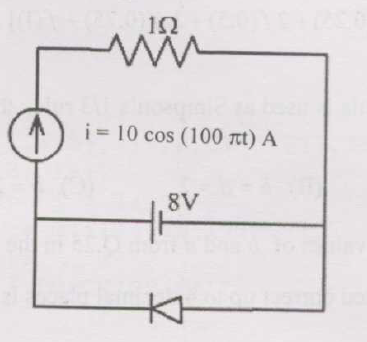
\includegraphics[width=0.6\columnwidth]{figs/C/fig1.png}
  \caption{Circuit}
  \label{fig:C/figs1.png}
\end{figure}
    \hfill{(GATE 2007 XE)}
    \begin{multicols}{4}
    \begin{enumerate}
        \item -28W
        \item 0W
        \item 64W
        \item 80W
    \end{enumerate}
    \end{multicols}
    \newpage

    \item An ideal transformer with 10 turns in primary and 30 turns in secondary has its primary connected to external circuits as shown. The current provided from the sinusoidal voltage source is:
    \begin{figure}[htbp]
  \centering
  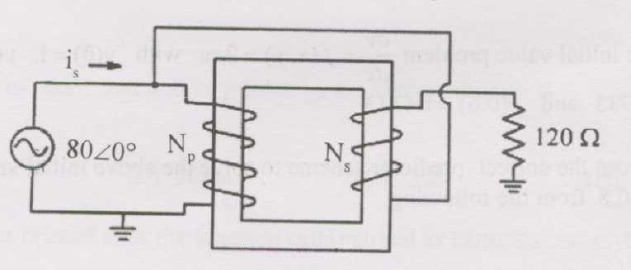
\includegraphics[width=0.6\columnwidth]{figs/C/fig2.png}
  \caption{Transformer}
  \label{fig:C/figs2.png}
\end{figure}

    \hfill{(GATE 2007 XE)}
    \begin{multicols}{4}
    \begin{enumerate}
        \item $0.67\angle 0^\circ$
        \item $2.0\angle 0^\circ$
        \item $2.67\angle 0^\circ$
        \item $10.67\angle 0^\circ$
    \end{enumerate}
    \end{multicols}

    \item In a three-phase, Y-connected squirrel cage induction motor, if $N_s$ is synchronous speed, $N_r$ is rotor speed and s is slip, then speeds of airgap field and rotor field w.r.t. stator structure will be respectively:
    \hfill{(GATE 2007 XE)}
    \begin{multicols}{4}
    \begin{enumerate}
        \item $N_s$, $N_s$
        \item $N_r$, $N_s$
        \item $N_r$, $N_r$
        \item $N_s$, $N_r$
    \end{enumerate}
    \end{multicols}

    \item The equivalent conductance of a forward biased diode at room temperature is:\\
    \hfill{(GATE 2007 XE)}
    \begin{multicols}{2}
    \begin{enumerate}
        \item constant
        \item proportional to V
        \item proportional to $V^2$
        \item proportional to $\exp(KV)$
    \end{enumerate}
\end{multicols}

    \item An 8-bit signed magnitude number $(10101010)_2$ represents the decimal:\\
    \hfill{(GATE 2007 XE)}
    \begin{multicols}{4}
    \begin{enumerate}
        \item -42
        \item -85
        \item -86
        \item -176
    \end{enumerate}
\end{multicols}

    \item A 10-bit DAC with full-scale $5\,V$ has resolution and step size respectively:\\
    \hfill{(GATE 2007 XE)}
    \begin{multicols}{2}
    \begin{enumerate}
        \item 0.0978\%, 500\,mV
        \item 0.0978\%, 4.88\,mV
        \item 0.195\%, 9.76\,mV
        \item 0.195\%, 500\,mV
    \end{enumerate}
\end{multicols}

\newpage
    \item A power source has open circuit voltage 24 V and short circuit current 16 A. Terminal characteristics shown below:
    \begin{figure}[htbp]
  \centering
  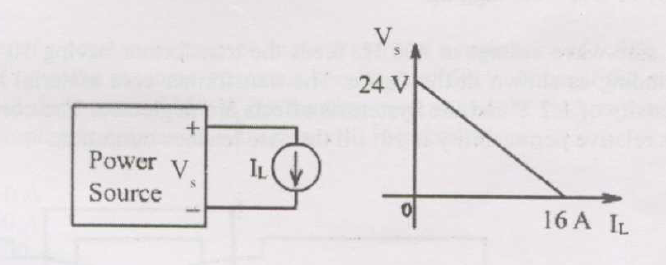
\includegraphics[width=0.6\columnwidth]{figs/C/fig3.png}
  \caption{Circuit}
  \label{fig:C/fig3.png}
\end{figure}
    \hfill{(GATE 2007 XE)}
    \begin{multicols}{2}
    \begin{enumerate}
        \item Load current = 16 A
        \item Source voltage = 24 V
        \item Load power = 96 W
        \item Load power = 384 W
    \end{enumerate}
\end{multicols}

    \item A 100 kVA, 11 kV/415 V transformer with 2\% winding resistance and 4\% leakage reactance. Voltage regulation at rated KVA, 0.8 pf lagging load is:
    \hfill{(GATE 2007 XE)}
    \begin{multicols}{4}
    \begin{enumerate}
        \item 2\%
        \item 4\%
        \item 4.8\%
        \item 6\%
    \end{enumerate}
\end{multicols}

    \item Source voltage of three-phase network is 11 kV. Line voltage at load end and phase angle w.r.t source voltage:
    \begin{figure}[htbp]
  \centering
  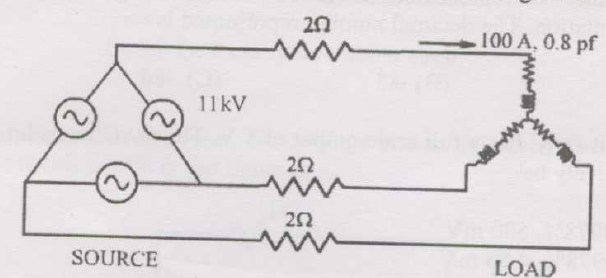
\includegraphics[width=0.6\columnwidth]{figs/C/fig4.png}
  \caption{Network}
  \label{fig:C/fig4.png}
\end{figure}
    
    \hfill{(GATE 2007 XE)}
    \begin{multicols}{2}
    \begin{enumerate}
        \item 10.7 kV, 0°
        \item 10.7 kV, 1.08° lagging
        \item 10.7 kV, 1.08° leading
        \item 11 kV, 1.08° lagging
    \end{enumerate}
\end{multicols}

\newpage

    \item A sine-wave voltage at 400 Hz feeds a transformer with 50 primary turns, core saturation flux density 1.2 T, core area 10 cm$^2$, relative permeability 1000. Max amplitude without saturation is:
    \begin{figure}[htbp]
  \centering
  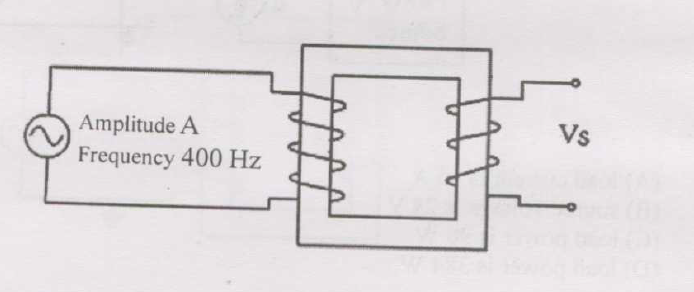
\includegraphics[width=0.6\columnwidth]{figs/C/fig5.png}
  \caption{Transformer}
  \label{fig:C/fig5.png}
\end{figure}
    \hfill{(GATE 2007 XE)}
    \begin{multicols}{4}
    \begin{enumerate}
        \item 24 V
        \item 48 V
        \item 75.4 V
        \item 150.8 V
    \end{enumerate}
\end{multicols}

    \item A 415 V/240 V, 1 kVA, 50 Hz transformer has leakage reactance 4\%. Leakage inductance of secondary winding is:
    \hfill{(GATE XE 2007)}
    \begin{multicols}{4}
    \begin{enumerate}
        \item 7.3 mH
        \item 21.9 mH
        \item 183 mH
        \item 2300 mH
    \end{enumerate}
    \end{multicols}

    \item Transformer with 100 turns primary and 50 turns secondary on C core with 1.0 mm airgap, core area 1.0 cm$^2$, primary connected to $v_p=10\cos (2000\pi t)$V. Peak MMF of primary winding is:
   \begin{figure}[htbp]
  \centering
  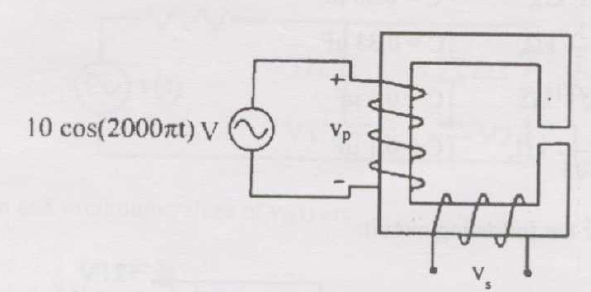
\includegraphics[width=0.6\columnwidth]{figs/C/fig6.png}
  \caption{Transformer}
  \label{fig:C/fig6.png}
\end{figure}
    \hfill{(GATE 2007 XE)}
    \begin{multicols}{4}
    \begin{enumerate}
        \item 126.65 AT
        \item 253.3 AT
        \item 314 AT
        \item 1000 AT
    \end{enumerate}
    \end{multicols}

\newpage

    \item PMDC generator armature resistance 0.5 $\Omega$, speed 600 rpm, voltage 60 V. When armature connected to 150 V DC source, starting current and line current at 1200 rpm are:\\
    \hfill{(GATE 2007 XE)}
    \begin{multicols}{4}
    \begin{enumerate}
        \item 120 A, 60 A
        \item 300 A, 60 A
        \item 120 A, 120 A
        \item 300 A, 120 A
    \end{enumerate}
\end{multicols}

    \item 4-pole DC machine with lap wound armature radius 14.2 cm, length 26.3 cm, poles cover 80\% armature, 39 coils 5 turns each, flux per pole is:\\
    \hfill{(GATE 2007 XE)}
    \begin{multicols}{4}
    \begin{enumerate}
        \item 15.95 mWb
        \item 31.9 mWb
        \item 39.9 mWb
        \item 63.8 mWb
    \end{enumerate}
\end{multicols}

    \item DC shunt motor at 1400 rpm fed by 220 V DC, line current 101 A, field resistance 220 $\Omega$, armature resistance 0.2 $\Omega$. Mechanical power developed

    \hfill{(GATE 2007 XE)}
    \begin{multicols}{4}
    \begin{enumerate}
        \item 22.22 kW
        \item 22 kW
        \item 20 kW
        \item 2 kW
    \end{enumerate}
\end{multicols}

    \item A transistor oscillator uses a 3-section RC phase shift circuit. Oscillation frequency 10 k rad/s, suitable R and C values are:
    \hfill{(GATE 2007 XE)}
    \begin{multicols}{2}
    \begin{enumerate}
        \item $R=3\,k\Omega$, $C=0.33\,\mu F$
        \item $R=1\,k\Omega$, $C=0.33\,\mu F$
        \item $R=\frac{1}{\sqrt{3}}\,k\Omega$, $C=0.1\,\mu F$
        \item $R=1\,k\Omega/\sqrt{3}$, $C=0.1\,\mu F$
    \end{enumerate}
    \end{multicols}

    \item For transistor circuit given, $\beta=50$, $C \to \infty$. The quiescent collector current $I_{CQ}$ is:
    \begin{figure}[htbp]
  \centering
  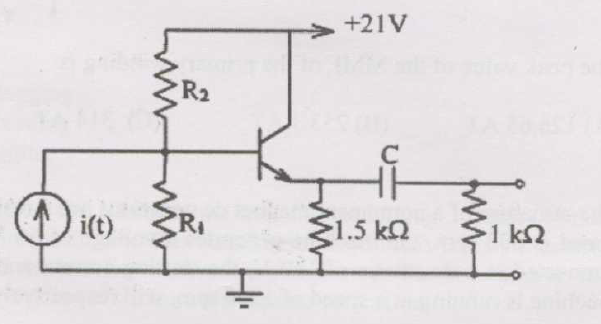
\includegraphics[width=0.6\columnwidth]{figs/C/fig7.png}
  \caption{Transistor Circuit}
  \label{fig:C/fig7.png}
\end{figure}
    \hfill{(GATE 2007 XE)}
    \begin{multicols}{4}
    \begin{enumerate}
        \item 7 mA
        \item 10 mA
        \item 14 mA
        \item 35 mA
    \end{enumerate}
    \end{multicols}
    
    \newpage 
    
    \item The CMOS circuit shown below represents:
    \begin{figure}[htbp]
  \centering
  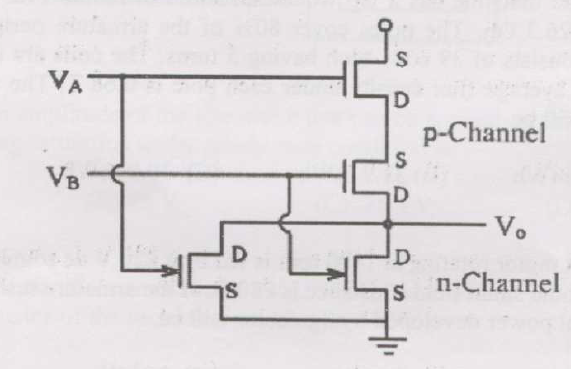
\includegraphics[width=0.6\columnwidth]{figs/C/fig8.png}
  \caption{CMOS circuit}
  \label{fig:C/fig8.png}
\end{figure}

    \hfill{(GATE 2007 XE)}
    \begin{multicols}{4}
    \begin{enumerate}
        \item AND gate
        \item NAND gate
        \item OR gate
        \item NOR gate
    \end{enumerate}
    \end{multicols}

    \item In the circuit below, $v(t) = 3\cos \omega t$, diode cut-in voltage 0.7 V, $V_1 = 2V$, $V_2=1V$. Max and min values of $v_o(t)$ are:
    \begin{figure}[htbp]
  \centering
  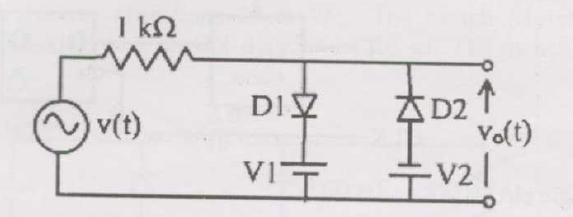
\includegraphics[width=0.6\columnwidth]{figs/C/fig9.png}
  \caption{Circuit}
  \label{fig:C/fig9.png}
\end{figure}
    \hfill{(GATE 2007 XE)}
    \begin{multicols}{4}
    \begin{enumerate}
        \item +2.3 V, -1.7 V
        \item +2.7 V, -1.7 V
        \item +1.3 V, -0.3 V
        \item +2.3 V, -1.3 V
    \end{enumerate}
    \end{multicols}

\newpage

    \item Given $v(t) = 2 \cos 2000 \pi t$ and ideal op-amp as shown, current $i_x(t)$ in 5 k$\Omega$ resistor is:
    \begin{figure}[htbp]
  \centering
  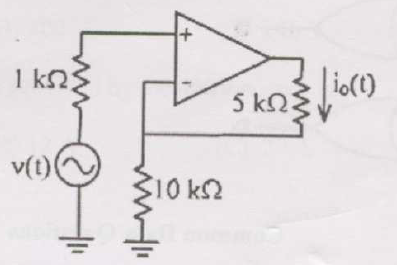
\includegraphics[width=0.6\textwidth]{figs/C/fig10.png}
  \caption{Circuit}
  \label{fig:C/fig10.png}
\end{figure}

    \hfill{(GATE 2007 XE)}
    \begin{multicols}{2}
    \begin{enumerate}
        \item 0.66 mA $\cos 2000 \pi t$
        \item 0.33 mA $\cos 2000 \pi t$
        \item 0.2 mA $\cos 2000 \pi t$
        \item 0.1 mA $\cos 2000 \pi t$
    \end{enumerate}
    \end{multicols}
    

    \item Simplified logic expression of circuit shown is:
    \begin{figure}[htbp]
  \centering
  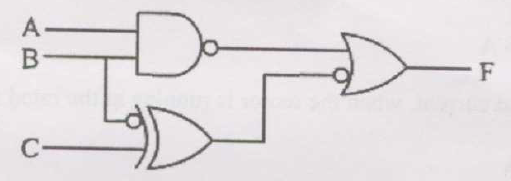
\includegraphics[width=0.6\columnwidth]{figs/C/fig11.png}
  \caption{Logic Gate}
  \label{fig:C/fig11.png}
\end{figure}

    \hfill{(GATE 2007 XE)}
    \begin{multicols}{4}
    \begin{enumerate}
        \item AB + BC
        \item AB + C
        \item A + B + C
        \item $\overline{A + B + C}$
    \end{enumerate}
    \end{multicols}

\newpage

    \item A D flip-flop is converted to T flip-flop by a logic circuit shown. The logic circuit is:
    \begin{figure}[htbp]
  \centering
  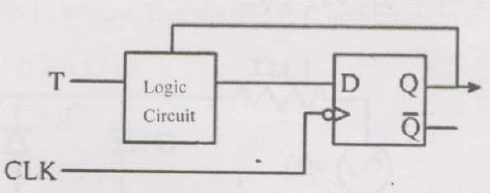
\includegraphics[width=0.6\columnwidth]{figs/C/fig12.png}
  \caption{Logic Circuit}
  \label{fig:C/fig12.png}
\end{figure}
    
    \hfill{(GATE 2007 XE)}
    \begin{multicols}{2}
    \begin{enumerate}
        \item \begin{center}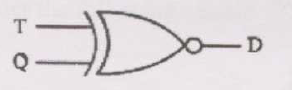
\includegraphics[width=0.5\columnwidth]{figs/C/fig22a.png}\end{center}
        \item \begin{center}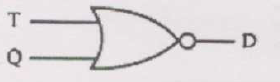
\includegraphics[width=0.5\columnwidth]{figs/C/fig22b.png}\end{center}
        \item \begin{center}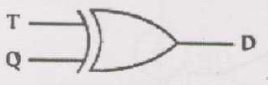
\includegraphics[width=0.5\columnwidth]{figs/C/fig22c.png}\end{center}
        \item \begin{center}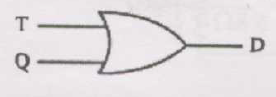
\includegraphics[width=0.5\columnwidth]{figs/C/fig22d.png}\end{center}
    \end{enumerate}
    \end{multicols}

    \item Three-phase, 4-pole, 400 V, 50 Hz, Y-connected induction motor with parameters $R_2=0.35 \Omega$, $X_2=0.25 \Omega$, $X_m=25 \Omega$. Stator impedance and iron loss neglected. Starting current for direct-on-line start is:

    \hfill{(GATE 2007 XE)}
    \begin{multicols}{4}
    \begin{enumerate}
        \item 542.36 A
        \item 659.83 A
        \item 939.4 A
        \item 1142.85 A
    \end{enumerate}
\end{multicols}

    \item Full load current at rated speed is:

    \hfill{(GATE 2007 XE)}
    \begin{multicols}{4}
    \begin{enumerate}
        \item 13.88 A
        \item 24.04 A
        \item 33.99 A
        \item 41.64 A
    \end{enumerate}
\end{multicols}

\newpage

    \item The switch $S_1$ turns on/off repeatedly at 20 kHz, with ON duration 20 $\mu$s. Switch \& diode ideal. The average load voltage $V_o$ is:
    \begin{figure}[htbp]
  \centering
  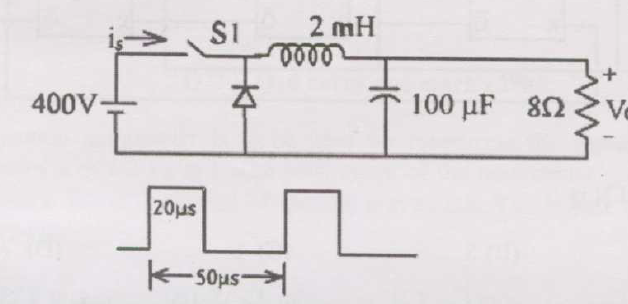
\includegraphics[width=0.6\columnwidth]{figs/C/fig13.png}
  \caption{Circuit}
  \label{fig:C/fig13.png}
\end{figure}
    \hfill{(GATE 2007 XE)}
    \begin{multicols}{4}
    \begin{enumerate}
        \item 667 V
        \item 400 V
        \item 240 V
        \item 160 V
    \end{enumerate}
    \end{multicols}
    

    \item Average source current $I_s$ provided by 400 V source is:
    \begin{figure}[htbp]
  \centering
  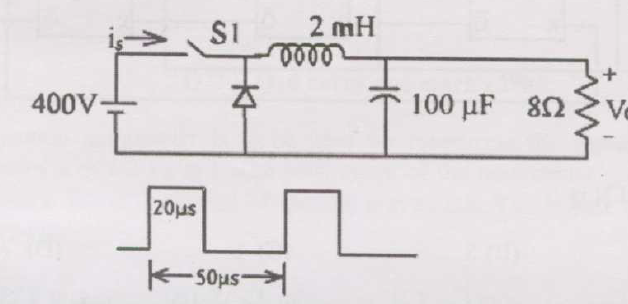
\includegraphics[width=0.6\columnwidth]{figs/C/fig13.png}
  \caption{Circuit}
  \label{fig:C/fig13.png}
\end{figure}
    \bigskip
    \hfill{(GATE 2007 XE)}
    \begin{multicols}{4}
    \begin{enumerate}
        \item 8 A
        \item 12 A
        \item 20 A
        \item 160 A
    \end{enumerate}
    \end{multicols}

    \newpage
    
    \item Divide by N counter using J-K flip-flops shown below. The value of N is:
    \begin{figure}[htbp]
  \centering
  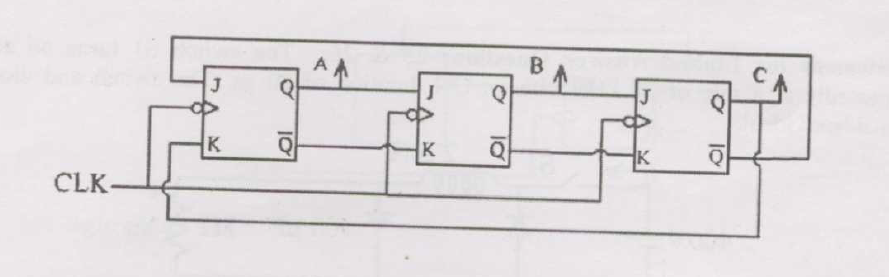
\includegraphics[width=0.9\columnwidth]{figs/C/fig14.png}
  \caption{Circuit}
  \label{C/fig14.png}
\end{figure}\\
    \hfill{(GATE 2007 XE)}
    \begin{multicols}{4}
    \begin{enumerate}
        \item 4
        \item 5
        \item 6
        \item 7
    \end{enumerate}
    \end{multicols}

    \item Counter output (Q27) goes to 3-to-8 decoder, LEDs as shown. LEDs that never glow are:
    \begin{figure}[htbp]
  \centering
  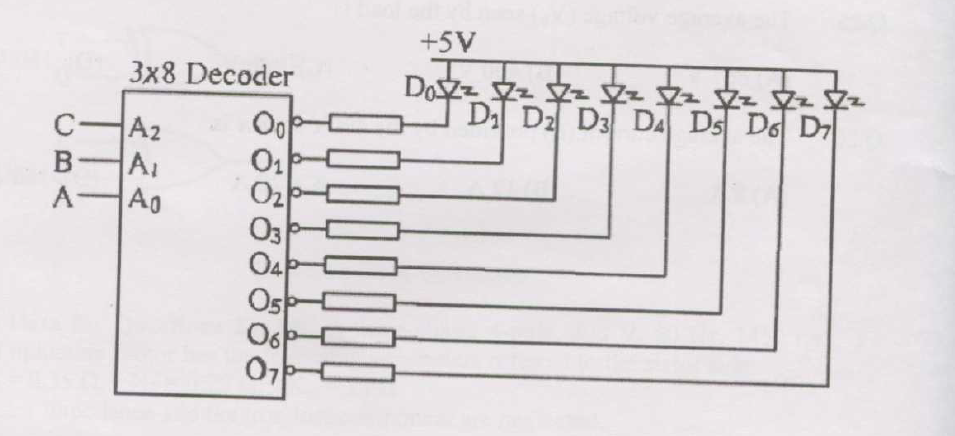
\includegraphics[width=0.7\columnwidth]{figs/C/fig15.png}
  \caption{LED Circuit}
  \label{fig:C/fig15.png}
\end{figure} \\
    \hfill{(GATE 2007 XE)}
    \begin{multicols}{4}
    \begin{enumerate}
        \item $D_0$ and $D_7$
        \item $D_0$ and $D_2$
        \item $D_2$ and $D_5$
        \item $D_5$ and $D_7$
    \end{enumerate}
    \end{multicols}

    \vspace{3\baselineskip}
    \begin{center}
    \textbf{\Large ---END OF SECTION---}
    \end{center}
\end{enumerate}

\newpage 

%-------------------Section-D------------------


\section*{Section D: Fluid Mechanics}
\vspace{2\baselineskip}
\begin{enumerate}
% ---------- Q1 ----------
\item A projection manometer measures the dynamic pressure of an airstream ($\rho = 1.2\,\text{kg/m}^3$). The manometric liquid is alcohol (specific gravity 0.8), least count 0.1 mm, $g = 10\,\text{m/s}^2$, water density $\rho = 1000\,\text{kg/m}^3$. The lowest measurable velocity is:
\hfill{(GATE 2007 XE)}

\begin{multicols}{4}
\begin{enumerate}

    \item $\sqrt{3}/2\,\text{m/s}$
    \item $2/\sqrt{3}\,\text{m/s}$
    \item $\sqrt{3}\,\text{m/s}$
    \item $2\,\text{m/s}$
\end{enumerate}
\end{multicols}


% ---------- Q2 ----------
\item The velocity of sound:  
\hfill{(GATE 2007 XE)}
\begin{multicols}{2}
\begin{enumerate}
    \item is a thermodynamic state variable
    \item is constant for a particular fluid
    \item depends on the velocity field
    \item depends on laminar or turbulent flow
\end{enumerate}
\end{multicols}

% ---------- Q3 ----------
\item The mass balance equation 

\begin{align*}
\frac{\partial \rho}{\partial t} 
+ \frac{\partial (\rho u)}{\partial x} 
+ \frac{\partial (\rho v)}{\partial y} 
= 0
\end{align*}

holds for:  
\hfill{(GATE 2007 XE)}
\begin{multicols}{2}
\begin{enumerate}
    \item steady/unsteady, compressible/incompressible
    \item steady/unsteady, compressible only
    \item steady/unsteady, incompressible only
    \item steady, compressible or incompressible
\end{enumerate}
\end{multicols}

% ---------- Q4 ----------

\item The non-dimensional number from specific heat c, thermal conductivity k, and viscosity $\mu$ is:  
\hfill{(GATE 2007 XE)}
\begin{multicols}{4}
\begin{enumerate}
    \item $\frac{k c_p}{\mu}$
    \item $\sqrt{\frac{k u}{c_p}}$
    \item $\frac{k \mu}{c_p}$
    \item $\frac{\mu c}{k}$
\end{enumerate}
\end{multicols}

% ---------- Q5 ----------

\item In a turbulent boundary layer, wall shear stress is  
$\tau_w = \mu \left.\frac{du}{dy}\right|_{\text{wall}}, $  
where $u$ is velocity parallel to the wall, $y$ is perpendicular. Here, $\mu$ denotes

\hfill{(GATE 2007 XE)}
\begin{multicols}{2}
\begin{enumerate}
    \item molecular viscosity
    \item turbulent eddy viscosity
    \item effective viscosity greater than molecular
    \item effective viscosity less than molecular
\end{enumerate}
\end{multicols}

% ---------- Q6 ----------
\newpage
\item Flow separation may occur if the flow is:

\hfill{(GATE 2007 XE)}
\begin{multicols}{2}
\begin{enumerate}
    \item viscous, positive streamwise pressure gradient
    \item viscous, negative streamwise pressure gradient
    \item inviscid, positive streamwise pressure gradient
    \item inviscid, negative streamwise pressure gradient
\end{enumerate}
\end{multicols}
% ---------- Q7 ----------

\item A solid sphere and hollow cube have the same surface area. The buoyancy force ratio (sphere:cube), fully submerged, is:  
\hfill{(GATE 2007 XE)}
\begin{multicols}{4}
\begin{enumerate}
    \item $\frac{\pi^2}{4}$
    \item $\frac{\pi}{6}$
    \item $\frac{\pi}{8}$
    \item $\frac{\pi}{67}$
\end{enumerate}
\end{multicols}

% ---------- Q8 ----------
\item For steady 2D incompressible flow, if temperature $T(x,y)$ is constant along a streamline, the streamline equation is:  
\hfill{(GATE 2007 XE)}
\begin{multicols}{4}
\begin{enumerate}
    \item $\frac{\partial T}{\partial x} = \frac{\partial T}{\partial y} \cdot \frac{dy}{dx}$
    \item $\frac{\partial T}{\partial x} \cdot \frac{dy}{dx} = \frac{\partial T}{\partial y}$
    \item $\frac{\partial T}{\partial y} \cdot \frac{dy}{dx} = \frac{\partial T}{\partial x}$
    \item $\frac{\partial T}{\partial y} = \frac{\partial T}{\partial x} \cdot \frac{dy}{dx}$
\end{enumerate}
\end{multicols}

% ---------- Q9 ----------
\item In a 2D laminar boundary layer with constant free-stream velocity, the signs of material acceleration (parallel, perpendicular to wall) near the wall are:

\hfill{(GATE 2007 XE)}
\begin{multicols}{4}
\begin{enumerate}
    \item $+$, $-$
    \item $-$, $+$
    \item $+$, $+$
    \item $-$, $-$
\end{enumerate}
\end{multicols}

% ---------- Q10 ----------
\item Water enters a pipe (area $A$) and branches into sections (areas $A_2$, $A_3$). Velocities at one instant: $V_1=2\,\text{m/s}$, $V_2=3\,\text{m/s}$, $V_3=5\,\text{m/s}$. At another, $V_1=3\,\text{m/s}$, $V_2=4\,\text{m/s}$. Find $V_3$:  
\begin{figure}[htbp]
  \centering
  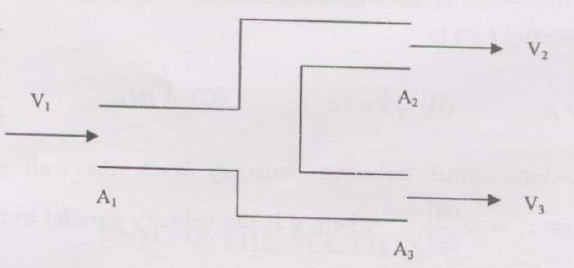
\includegraphics[width=0.6\columnwidth]{figs/D/fig1.png}
  \caption{Pipe Diagram}
  \label{fig:D/fig1.png}
\end{figure}
\hfill{(GATE 2007 XE)}
\begin{multicols}{4}
\begin{enumerate}
    \item $5\,\text{m/s}$
    \item $6\,\text{m/s}$
    \item $7\,\text{m/s}$
    \item $8\,\text{m/s}$
\end{enumerate}
\end{multicols}

% ---------- Q11 ----------
\newpage
\item In 2D incompressible irrotational flow, $u = 2x + 3y$. The $y$-component of velocity is:  
\hfill{(GATE 2007 XE)}
\begin{enumerate}[label=\alph*)]
    \item $2y - 3x$
    \item $2y + 3x$
    \item $-2y + 3x$
    \item $-2y - 3x$
\end{enumerate}

% ---------- Q12 ----------

\item For steady 2D flow with $u=6y$, $v=0$ ($y$ is vertical distance), the angular velocity and shear strain rate are:
\hfill{(GATE 2007 XE)}
\begin{multicols}{4}
\begin{enumerate}
    \item $-3$, $3$
    \item $3$, $-3$
    \item $3$, $-6$
    \item $-6$, $3$
\end{enumerate}
\end{multicols}

% ---------- Q13 ----------

\item In steady 2D incompressible flow, the stream function $\psi$ obeys:  

$\frac{\partial^2 \psi}{\partial x^2} + \frac{\partial^2 \psi}{\partial y^2} = 4.$ 
A solution is:
\hfill{(GATE 2007 XE)}
\begin{multicols}{4}
\begin{enumerate}
    \item $\psi = x^2 + y^2$
    \item $\psi = y^2 - x^2$
    \item $\psi = xy$
    \item $\psi = x + y$
\end{enumerate}
\end{multicols}

% ---------- Q14 ----------

\item A uniform stream of ideal fluid (velocity $U$, pressure $p$) flows past a circular cylinder. Wall velocity is $V = 2U \sin \theta$. Pressure coefficient $C_p = \frac{P - P_\infty}{0.5 \rho U^2}$. The minimum $C_p$ on the cylinder is:  
\begin{figure}[htbp]
  \centering
  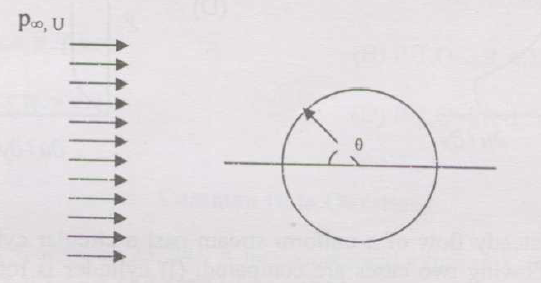
\includegraphics[width=0.6\columnwidth]{figs/D/fig2.png}
  \caption{Circular Cylinder}
  \label{fig:D/fig2.png}
\end{figure}\\
\hfill{(GATE 2007 XE)}
\begin{multicols}{4}
\begin{enumerate}
    \item $1$
    \item $-1$
    \item $-3$
    \item $-4$
\end{enumerate}
\end{multicols}
% ---------- Q15 ----------
\newpage
\item A model (length 20 cm) studies water flow ($v=10^{-6}\,\text{m}^2/\text{s}$) in a 5 m channel. The model’s kinematic viscosity should be:  
\hfill{(GATE 2007 XE)}
\begin{multicols}{4}
\begin{enumerate}
    \item $4 \times 10^{-6}$
    \item $8 \times 10^{-6}$
    \item $4 \times 10^{-7}$
    \item $8 \times 10^{-7}$
\end{enumerate}
\end{multicols}

% ---------- Q16 ----------

\item Water flows through a 5 cm diameter tube at $\pi\,\text{kg/s}$, $\mu=0.001\,\text{Ns/m}^2$, $\rho = 1000\,\text{kg/m}^3$. Darcy friction factor: $f=64/\text{Re}$ (laminar), $f=0.316 \text{Re}^{-0.25}$ (turbulent). Approximate pressure drop per unit length is:  
\hfill{(GATE 2007 XE)}
\begin{multicols}{4}
\begin{enumerate}
    \item $20\,\text{Pa/m}$
    \item $120\,\text{Pa/m}$
    \item $480\,\text{Pa/m}$
    \item $960\,\text{Pa/m}$
\end{enumerate}
\end{multicols}

% ---------- Q17 ----------
\item Constant pressure boundary layer over a 3 m plate, $U=60\,\text{m/s}$, $\rho=1.23\,\text{kg/m}^3$, $\mu=1.79 \times 10^{-5}\,\text{Ns/m}^2$. Transition at $x_{cr}=0.1\,\text{m}$. If $U=120\,\text{m/s}$, new $x_{cr}$ is:

\hfill{(GATE 2007 XE)}
\begin{multicols}{4}
\begin{enumerate}
    \item $0.2\,\text{m}$
    \item $0.1\,\text{m}$
    \item $0.05\,\text{m}$
    \item $0.005\,\text{m}$
\end{enumerate}
\end{multicols}
% ---------- Q18 ----------

\item For a laminar boundary layer with constant free-stream velocity ($\frac{dp}{dx}$=0), the variation of $\partial u / \partial y$ with $y$ is:  
\hfill{(GATE 2007 XE)}

\begin{multicols}{2}
\begin{enumerate}
    \item \quad 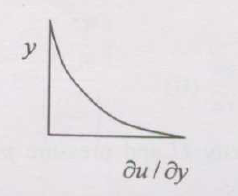
\includegraphics[width=0.3\columnwidth]{figs/D/fig18a.png}
    \item \quad 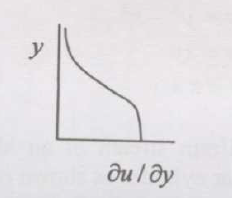
\includegraphics[width=0.3\columnwidth]{figs/D/fig18b.png}
    \item \quad 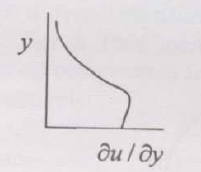
\includegraphics[width=0.3\columnwidth]{figs/D/fig18c.png}
    \item \quad 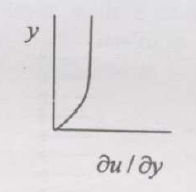
\includegraphics[width=0.3\columnwidth]{figs/D/fig18d.png}
\end{enumerate}
\end{multicols}

% ---------- Q19 ----------
\item Steady viscous flow past a cylinder: (I) slow rotation, (II) no rotation. Which is true?  

P: Lift force zero in (I) \quad Q: Lift force zero in (II) \\
R: Drag force non-zero in (I) \quad S: Drag force zero in (II) \\
\hfill{(GATE 2007 XE)}

\begin{multicols}{4}
\begin{enumerate}
    \item P, Q, R
    \item P, R, S
    \item P, S
    \item Q, R
\end{enumerate}
\end{multicols}

% ---------- Q20 ----------

\item Orifice plate (60 mm diameter, discharge coefficient 0.6) measures air flow ($\rho = 1.2\,\text{kg/m}^3$, $\mu=1.8 \times 10^{-5}\,\text{kg m}^{-1}\text{s}^{-1}$) in a 100 mm pipe. Manometer reading 180 mm of water. Air flow rate is:  
\hfill{(GATE 2007 XE)}
\begin{multicols}{4}
\begin{enumerate}
    \item $0.3\,\text{m}^3/\text{s}$
    \item $0.1\,\text{m}^3/\text{s}$
    \item $0.01\,\text{m}^3/\text{s}$
    \item $0.003\,\text{m}^3/\text{s}$
\end{enumerate}
\end{multicols}

% ---------- Q21 ----------
\newpage
\item Airstream velocity ($\rho=1.0\,\text{kg/m}^3$) measured with a Pitot-static tube, manometer difference 2 cm of water. Velocity is:  
\hfill{(GATE 2007 XE)}

\begin{multicols}{4}
\begin{enumerate}
    \item $0.02\,\text{m/s}$
    \item $2.0\,\text{m/s}$
    \item $10\,\text{m/s}$
    \item $20\,\text{m/s}$
\end{enumerate}
\end{multicols}

% ---------- Q22 ----------
\item Match the following columns using the most appropriate combinations:  

\begin{center}
\begin{tabular}{ll}
    \textbf{Group I} & \textbf{Group II} \\
    P. Ferrite & 1. Hexagonal Close Packed (HCP) \\
    Q. Austenite & 2. Body Centered Cubic (BCC) \\
    R. Martensite & 3. Body Centered Tetragonal (BCT) \\
    & 4. Face Centered Cubic (FCC)
\end{tabular}
\end{center}

Correct matching is:  
\hfill{(GATE 2007 XE)}
\begin{multicols}{2}
\begin{enumerate}
    \item P-3, Q-4, R-1, S-5
    \item P-1, Q-2, R-4, S-3
    \item P-4, Q-5, R-2, S-3
    \item P-2, Q-4, R-1, S-3
\end{enumerate}
\end{multicols}

% ---------- Q23 ----------
\item A line source and sink of unit strength at $x=-1$ and $x=+1$. Velocity at (0,1) in Cartesian unit vectors $\mathbf{i}$, $\mathbf{j}$ is:  
\hfill{(GATE 2007 XE)}

\begin{multicols}{4}
\begin{enumerate}
    \item $0\mathbf{i} + 0\mathbf{j}$
    \item $\frac{1}{2\pi} \mathbf{i} + 0 \mathbf{j}$
    \item $0 \mathbf{i} + \frac{1}{2\pi} \mathbf{j}$
    \item $\frac{1}{\pi} \mathbf{i} + 0 \mathbf{j}$
\end{enumerate}
\end{multicols}

% ---------- Q24 ----------

\item Source and sink in a uniform stream correspond to:  
\hfill{(GATE 2007 XE)}

\begin{multicols}{2}
\begin{enumerate}
    \item doublet
    \item flow over circular cylinder
    \item flow over Rankine half-body
    \item flow over Rankine oval
\end{enumerate}
\end{multicols}
% ---------- Q25 ----------

\item A motorboat cruises at 10 m/s. A 180 kW pump sucks water at 1 m$^3$/s and ejects it at 10 m/s relative to the lake. Total drag on the boat is:  

\begin{figure}[htbp]
  \centering
  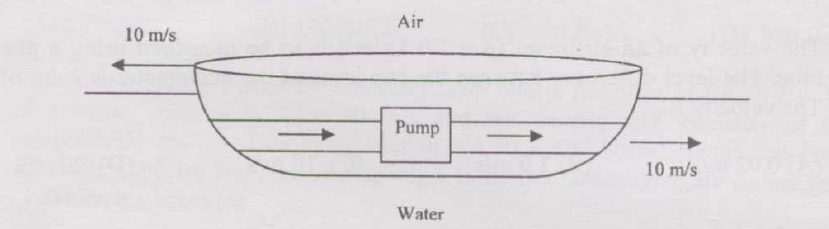
\includegraphics[width=1.0\columnwidth]{figs/D/fig3.png}
  \caption{Motor Boat}
  \label{fig:D/fig3.png}
\end{figure}
\hfill{(GATE 2007 XE)}
\begin{multicols}{4}
\begin{enumerate}
    \item $30\,\text{kN}$
    \item $20\,\text{kN}$
    \item $10\,\text{kN}$
    \item $0\,\text{kN}$
\end{enumerate}
\end{multicols}

% ---------- Q26 ----------
\item From Q25, Power utilized for propelling the boat is:  
\hfill{(GATE 2007 XE)}
\begin{multicols}{4}
\begin{enumerate}
    \item $130\,\text{kW}$
    \item $100\,\text{kW}$
    \item $80\,\text{kW}$
    \item $30\,\text{kW}$
\end{enumerate}
\end{multicols}
% ---------- Q27 ----------

\item Fully developed laminar flow in a pipe (radius $R$) with axial velocity:  
\[
u(r) = \frac{-R^2}{4\mu} \frac{dp}{dx} \left(1 - \frac{r^2}{R^2}\right).
\]  
Wall shear stress magnitude $\tau_{wall}$ is:  
\hfill{(GATE 2007 XE)}
\begin{multicols}{4}
\begin{enumerate}
    \item $\frac{4 \mu U_m}{R}$
    \item $\rho u R$
    \item $\frac{\mu U_m}{R}$
    \item $-\frac{R}{2} \frac{dp}{dx}$
\end{enumerate}
\end{multicols}
% ---------- Q28 ----------

\item Local friction factor $C_f$ with $y = \frac{dp}{dx}$ is:  
\hfill{(GATE 2007 XE)}
\begin{multicols}{4}
\begin{enumerate}
    \item $\frac{16 \mu^2}{\rho^2 R^3 y}$
    \item $\frac{24 \mu^2}{\rho^2 R^3 y}$
    \item $\frac{64 \mu^2}{\rho^2 R^3 y}$
    \item $\frac{2 \mu y}{\rho R}$
\end{enumerate}
\end{multicols}


\end{enumerate}

    \begin{center}
    \textbf{\Large ---END OF SECTION---}
    \end{center}




    %----------------------Section-E-----------------------
\newpage
\section*{Section E: Material Science}

\begin{enumerate}
\vspace{2\baselineskip}

% ---------- Q1 ----------

\item High bond energy in a crystal leads to:  

\hfill{(GATE 2007 XE)}
\begin{multicols}{2}
\begin{enumerate}
    \item high elastic modulus, low melting point, high coefficient of thermal expansion
    \item low elastic modulus, high melting point, low coefficient of thermal expansion
    \item high elastic modulus, high melting point, low coefficient of thermal expansion
    \item low elastic modulus, low melting point, high coefficient of thermal expansion
\end{enumerate}
\end{multicols}
% ---------- Q2 ----------
\item Which oxide does NOT form glass by itself?  
\hfill{(GATE 2007 XE)}
\begin{multicols}{4}
\begin{enumerate}
    \item $SiO_{2}$
    \item $B_2$$O_3$
    \item $P_2$$O_5$
    \item $Al_2$$O_3$
\end{enumerate}
\end{multicols}

% ---------- Q3 ----------

\item Diffusion mechanism with lowest activation energy is:  
\hfill{(GATE 2007 XE)}
\begin{multicols}{2}
\begin{enumerate}
    \item Lattice diffusion
    \item Grain boundary diffusion
    \item Surface diffusion
    \item Diffusion through dislocations
\end{enumerate}
\end{multicols}

% ---------- Q4 ----------

\item  In tensile test, necking starts at:  
\hfill{(GATE 2007 XE)}
\begin{multicols}{2}
\begin{enumerate}
    \item lower yield point
    \item upper yield point
    \item ultimate tensile stress
    \item proof stress
\end{enumerate}
\end{multicols}

% ---------- Q5 ----------

\item Si is added to transformer grade steel to:  
\hfill{(GATE 2007 XE)}
\begin{multicols}{2}
\begin{enumerate}
    \item decrease magnetic permeability
    \item decrease electrical resistivity
    \item improve ductility
    \item increase magnetic permeability
\end{enumerate}
\end{multicols}
% ---------- Q6 ----------

\item According to galvanic series, the most active metal among: Mg, Zn, Sn, Al is:

\hfill{(GATE 2007 XE)}
\begin{multicols}{4}
\begin{enumerate}
    \item Mg
    \item Zn
    \item Sn
    \item Al
\end{enumerate}
\end{multicols}

% ---------- Q7 ----------

\item Enthalpy of vacancy formation in Cu is 120 kJ/mol. Equilibrium fraction of vacant lattice sites in Cu at 1000 K is: 
\hfill{(GATE 2007 XE)}
\begin{multicols}{4}
\begin{enumerate}
    \item $1.35 \times 10^{-8}$
    \item $5.39 \times 10^{-7}$
    \item $7.76 \times 10^{-6}$
    \item $2.58 \times 10^{-9}$
\end{enumerate}
\end{multicols}

% ---------- Q8 ----------
\newpage
\item Metal melting point 1000 K, enthalpy of melting $2.0 \times 10^9$ J/m$^3$, solid-liquid interface energy 0.5 J/m$^2$. Radius of critical nucleus during solidification at 900 K is:  
\hfill{(GATE 2007 XE)}
\begin{multicols}{4}
\begin{enumerate}
    \item 10.0 nm
    \item 5.0 nm
    \item 5.0 $\mu$m
    \item 2.5 nm
\end{enumerate}
\end{multicols}
% ---------- Q9 ----------

\item  In binary system A-B at 1 atm, parameters independently varied in two phase $(\alpha+\beta)$ region are:  
\hfill{(GATE 2007 XE)}
\begin{multicols}{2}
\begin{enumerate}
    \item composition of $\alpha$ phase and temperature
    \item composition of $\alpha$ and $\beta$ phases
    \item either composition of $\alpha$ or $\beta$ phase or temperature
    \item temperature only
\end{enumerate}
\end{multicols}
% ---------- Q10 ----------

\item Cd$^{++}$ doped NaCl crystal has higher conductivity at room temp due to:  \\

\hfill{(GATE 2007 XE)}
\begin{multicols}{2}
\begin{enumerate}
    \item lower activation energy for cation movement
    \item increase in cation vacancy concentration
    \item introduction of holes in crystal
    \item increase in anion vacancy concentration
\end{enumerate}
\end{multicols}

% ---------- Q11 ----------

\item Match heat treatments (P, Q, R, S) with microstructure (1-5) in hypoeutectoid steel: 

\hfill{(GATE 2007 XE)}
\begin{tabular}{|c|c|c|}
     \hline
     \textbf{Mineral} & \textbf{Modal abundance \brak{\%}} & \textbf{Partition coefficient}\\
     \hline
     Clinopyroxene & $45$ & $0.506$ \\
      \hline
      Orthopyroxene & $40$ & $0.42$ \\
      \hline
      Olivine & $10$ & $0.045$ \\
      \hline
      Plagioclase & $05$ & $0.019$ \\
      \hline
\end{tabular}
\begin{multicols}{2}
\begin{enumerate}
    \item P-4, Q-1, R-3, S-2
    \item P-5, Q-1, R-3, S-2
    \item P-1, Q-4, R-2, S-3
    \item P-2, Q-5, R-3, S-4
\end{enumerate}
\end{multicols}

% ---------- Q12 ----------

\item Second peak in powder X-ray diffraction pattern of FCC crystal at Bragg angle $23.21^\circ$ with Cu-K$\alpha$ wavelength 0.154 nm. Lattice parameter (nm) is:

\hfill{(GATE 2007 XE)}
\begin{multicols}{4}
\begin{enumerate}
    \item 0.391
    \item 0.338
    \item 0.276
    \item 0.437
\end{enumerate}
\end{multicols}

% ---------- Q13 ----------
\newpage
\item  Which direction lies in (111) plane?  
\hfill{(GATE 2007 XE)}
\begin{multicols}{4}
\begin{enumerate}
    \item (211)
    \item (110)
    \item (100)
    \item (112)
\end{enumerate}
\end{multicols}
% ---------- Q14 ----------

\item Yield strength varies with grain size $d$ as:  
\hfill{(GATE 2007 XE)}
\begin{multicols}{4}
\begin{enumerate}
    \item $d^{-1/2}$
    \item $d^{-1}$
    \item $d$
    \item $d^{1/2}$
\end{enumerate}
\end{multicols}
% ---------- Q15 ----------

\item  Toughening mechanism NOT contributing in SiC whisker reinforced alumina composite:  
\hfill{(GATE 2007 XE)}
\begin{multicols}{2}
\begin{enumerate}
    \item crack tip deflection
    \item transformation toughening
    \item bridging across crack face
    \item energy absorbed during whisker pull-out
\end{enumerate}
\end{multicols}

% ---------- Q16 ----------

\item Match experimental techniques (P, Q, R, S) with applications (1-5):  

\hfill{(GATE 2007 XE)}
\begin{table}[htbp]
  \centering
  \caption{Table-3}
  \label{table3}
  \begin{tabular}{cc}
  \textbf{Processing Technique} & \textbf{Producct} \\ \\
    P. Calendering & 1. Pipes \\
    Q. Extrusion & 2. Disposable cups \\
    R. Injection moulding & 3. Sheets \\
    S. Thermoforming & 4. Nylon gears \\
  \end{tabular}
\end{table}
\begin{multicols}{2}
\begin{enumerate}
    \item P-2, Q-3, R-1, S-5
    \item P-4, Q-3, R-5, S-3
    \item P-4, Q-3, R-1, S-2
    \item P-2, Q-4, R-1, S-5
\end{enumerate}
\end{multicols}

% ---------- Q17 ----------

\item  Match polymers (P, Q, R, S) with applications (1-5):    
\hfill{(GATE 2007 XE)}

\begin{center}
\begin{tabular}{|c|c|c|}
    \hline
    Task & Task time (Seconds) & Immediate predecessor(s) \\
    \hline
    P & 20 & - \\ \hline
    Q & 25 & P \\  \hline
    R & 10 & Q \\ \hline
    S & 15 & Q \\ \hline 
    T & 25 & R, S \\    \hline
\end{tabular}
\end{center}
\begin{multicols}{2}
\begin{enumerate}
    \item P-2, Q-1, R-4, S-3
    \item P-4, Q-1, R-3, S-2
    \item P-3, Q-1, R-5, S-4
    \item P-3, Q-1, R-5, S-2
\end{enumerate}
\end{multicols}

% ---------- Q18 ----------
\newpage
\item  Match materials (P, Q, R, S) with applications (1-5):  
\begin{table}[h!]
\centering
\begin{tabular}{|c|c|c|c|}
\hline
\textbf{Pressure} & \textbf{Temperature} & \multicolumn{2}{c|}{\textbf{Specific enthalpy}} \\ \cline{3-4} 
\textbf{(kPa)} & \textbf{($^\circ$C)} & $h_f$ (kJ/kg) & $h_g$ (kJ/kg) \\ \hline
150.9 & $-20$ & 17.82 & 178.74 \\ \hline
500 & 15.6 & 50.64 & 195.01 \\ \hline
\end{tabular}
\end{table}

\hfill{(GATE 2007 XE)}
\begin{multicols}{2}
\begin{enumerate}
    \item P-3, Q-5, R-1, S-2
    \item P-3, Q-5, R-4, S-2
    \item P-5, Q-4, R-1, S-2
    \item P-3, Q-5, R-4, S-1
\end{enumerate}
\end{multicols}
% ---------- Q19 ----------

\item  Optical transparency of a single crystal depends on:  
\hfill{(GATE 2007 XE)}
\begin{multicols}{2}
\begin{enumerate}
    \item Band gap
    \item Lattice parameter
    \item Crystal structure
    \item Work function
\end{enumerate}
\end{multicols}

% ---------- Q20 ----------
\item Drift mobility of electrons in intrinsic region of doped semiconductor as function of temperature:  
\hfill{(GATE 2007 XE)}
\begin{multicols}{2}
\begin{enumerate}
    \item limited by ionized impurity scattering
    \item limited by phonon scattering
    \item limited by point defects\\
    \item remains unaffected
\end{enumerate}
\end{multicols}

% ---------- Q21 ----------
\item  Zn$Fe_2$$O_4$ has inverse spinel structure. Atomic numbers of Zn, Fe, O are 30, 26, 8 respectively. Net magnetic moment per formula unit in Bohr magnetons ($\mu_B$) is:

\hfill{(GATE 2007 XE)}
\begin{multicols}{4}
\begin{enumerate}
    \item 2 $\mu_B$
    \item 1 $\mu_B$
    \item 4 $\mu_B$
    \item 0 $\mu_B$
\end{enumerate}
\end{multicols}

% ---------- Q22 ----------

\item $Nb_3$Sn is widely used in superconducting magnets because

\hfill{(GATE 2007 XE)}
\begin{multicols}{2}
\begin{enumerate}
    \item Type I superconductor
    \item Type II superconductor with large critical magnetic field
    \item $T_c$ above helium boiling point
    \item It is an intermetallic
\end{enumerate}
\end{multicols}

% ---------- Q23 ----------
\newpage
\item  Mo has BCC with lattice parameter 0.315 nm, atomic mass 96. Mo–Mo nearest neighbor distance (nm) is: 
\hfill{(GATE 2007 XE)}
\begin{multicols}{4}
\begin{enumerate}
    \item 0.223
    \item 0.273
    \item 0.136
    \item 0.1575
\end{enumerate}
\end{multicols}

% ---------- Q24 ----------
\item  Theoretical density of Mo (kg/m$^3$) is:  
\hfill{(GATE 2007 XE)}
\begin{multicols}{4}
\begin{enumerate}
    \item 20400
    \item 2550
    \item 10200
    \item 5100
\end{enumerate}
\end{multicols}

% ---------- Q25 ----------

\item  A continuous carbon fiber reinforced epoxy composite has 40 vol\% carbon fibers. Elastic modulus of fibers 400 GPa, epoxy 2.4 GPa. Density of fiber 1800 kg/m$^3$, epoxy 1200 kg/m$^3$. Density of composite (kg/m$^3$) is:  

\hfill{(GATE 2007 XE)}
\begin{multicols}{4}
\begin{enumerate}
    \item 1440
    \item 1200
    \item 1800
    \item 1340
\end{enumerate}
\end{multicols}
% ---------- Q26 ----------

\item Specific modulus of elasticity of composite in longitudinal direction is:  

\hfill{(GATE 2007 XE)}
\begin{multicols}{2}
\begin{enumerate}
    \item 2.76 MPa$\cdot$m$^3$/kg
    \item 112.11 GPa
    \item 161.44 GPa
    \item 112.11 MPa$\cdot$m$^3$/kg
\end{enumerate}
\end{multicols}
% ---------- Q27 ----------

\item  Intrinsic carrier density in Si at 300 K is $1.45 \times 10^{16}$ m$^{-3}$. Sample doped with 1 ppm As. Density of Si 2330 kg/m$^3$, atomic wt 28. Number of As atoms per m$^3$ is:  

\hfill{(GATE 2007 XE)}
\begin{multicols}{4}
\begin{enumerate}
    \item $5.01 \times 10^{22}$
    \item $5.01 \times 10^{26}$
    \item $5.01 \times 10^{19}$
    \item $3.929 \times 10^{23}$
\end{enumerate}
\end{multicols}

% ---------- Q28 ----------

\item Assuming all impurities ionized, hole concentration per m$^3$ is:  
\hfill{(GATE 2007 XE)}
\begin{multicols}{2}
\begin{enumerate}
    \item $2.894 \times 10^{-7}$
    \item $4.197 \times 10^{0}$
    \item $4.197 \times 10^{5}$
    \item $4.197 \times 10^{12}$
\end{enumerate}
\end{multicols}

    \vspace{3\baselineskip}
    \begin{center}
    \textbf{\Large ---END OF SECTION---}
    \end{center}

\end{enumerate}

\end{document}
